%----------------------------------------------------------------------------
\chapter{\bevezetes}
%----------------------------------------------------------------------------

\begin{figure}[!ht]
    \centering
    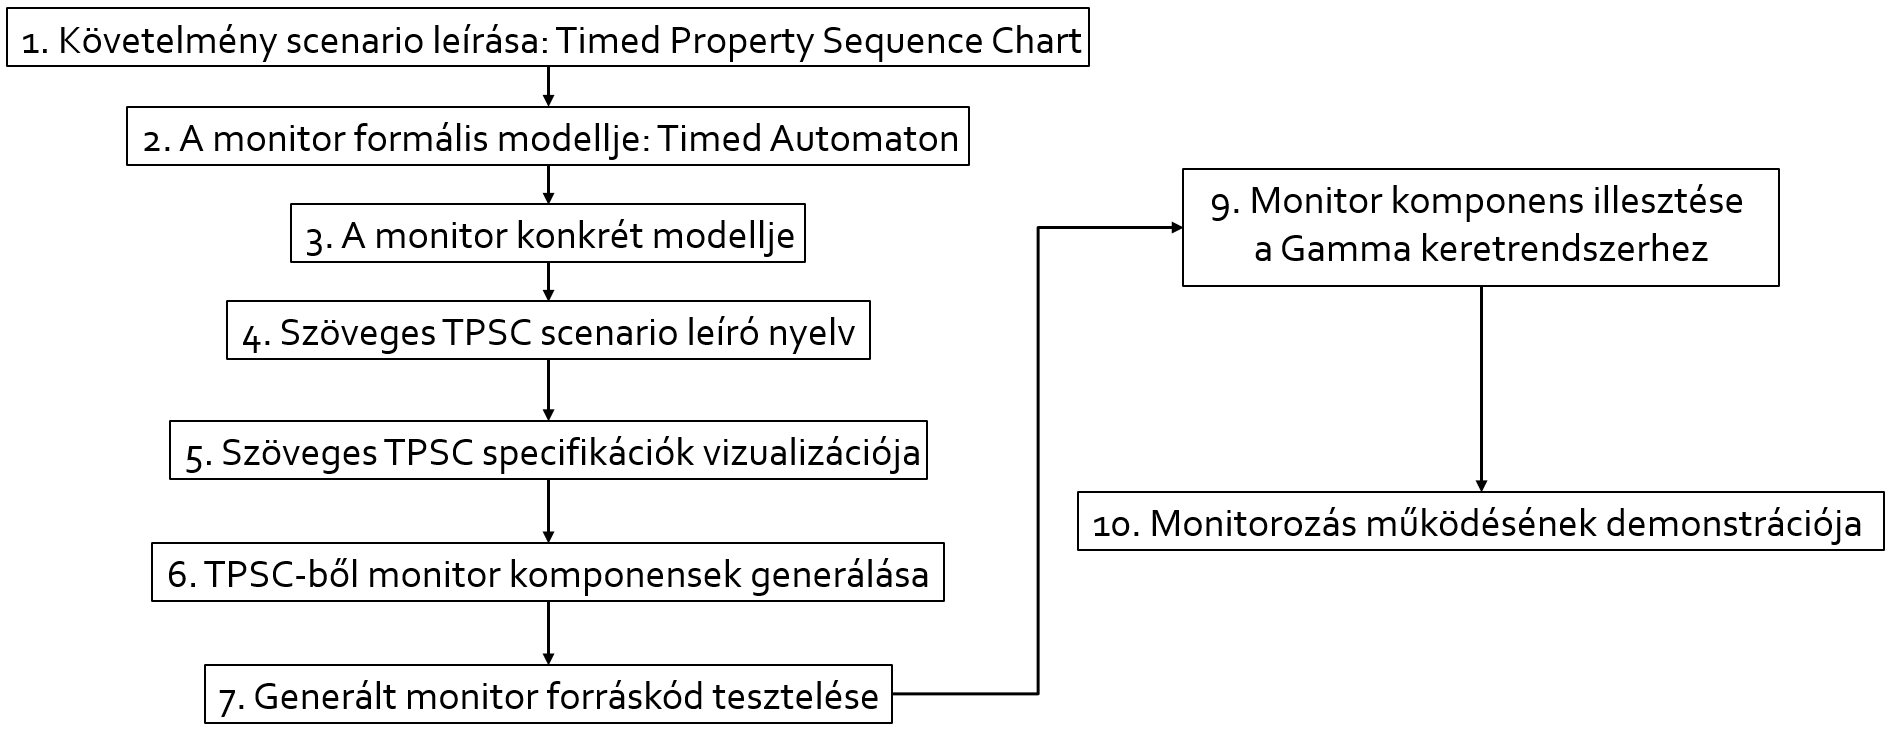
\includegraphics[width=150mm, keepaspectratio]{figures/generation_plan.png}
    \caption{Monitor generátor kibővítése.}
\end{figure}

Diplomamunkám során az volt a cél, hogy a „Monitor komponensek generálása kontextusfüggő viselkedés ellenőrzése” című szakdolgozatom során elkészített monitor komponens generátort kibővítsem úgy, hogy támogassa időzítési feltételek megadását.
A monitor generálás terve látható a 1.1. ábrán.
Az Önálló laboratórium keretében az volt a feladatom, hogy a szakdolgozat során definiált szöveges PSC diagram leíró nyelvet kibővitsem a TPSC elemeivel.
Ezután az automata generátort kell úgy kibővíteni, hogy a TPSC diagramokból tudjon TA automatákat generálni.
Egy monitor forráskód generátor pedig az automata alapján elkészítheti a monitor forráskódját.

A szöveges TPSC scenario leírásához el kell készítenünk a diagram vizualizációját, hogy grafikusan megtekinthessük a definiált szcenáriót.
Ehhez felhasználható a "Modell alapú rendszertervezés" tárgy keretében készített PSC diagram szerkesztő alkalmazás.
A következő a generált monitor forráskód tesztelése, majd ezután ezt illeszük a Gamma keretrendszerhez.
Ezzel az a célunk, hogy elosztott komponens alapú rendszerek szimulációja közben monitorozható legyen a TPSC üzenet szekvencia specifikáció teljesülése illetve az ebben rögzített tulajdonságok megsértése.

A Diplomatervezés 1 tárgy keretében elkészítettem a monitor forráskód generátort és elkezdtem annak tesztélését.
A hátramaradó feladatok közé tartozik a tesztelés befejezése, a diagramok vizualizációja és a monitor komponens illesztése a Gamma keretrendszerhez.

A dolgozatomat a háttérismeretek összefoglalásával kezdem.
Előszőr bemutatom a legelterjetebb formalizmusokat, amelyek időfüggő viselkedés specifikálására szolgálnak.
Ezután a TPSC formalizmust mutatom be és a felhasznált technológiákat.
A dolgozatomat a kivőbített szöveges TPSC leíró nyelv bemutatásával folytatom.
Ezt a TPSC specifikációk vizualizációjáról szoló fejezet követi.

A következő fejezet a monitor forráskód generálásról szól és annak teszteléséről.
Ezt követi egy fejezet, amely a monitor komponens illesztését mutatja be a Gamma keretrendszerhez és elosztott komponensúű rendszerek monitorozását.
A dolgozatomat egy összefoglalóval zárom.